\documentclass[10pt,twocolumn]{article}

% ----------------------------------------------------------------- packages
\usepackage[letterpaper,margin=0.85in,columnsep=0.28in]{geometry}
\usepackage{times}               % Times text, Computer Modern math (available in every TeX distribution)
\renewcommand{\ttdefault}{cmtt}  % CM typewriter: present even in minimal TeX installs
\usepackage{amsmath,amssymb}
\usepackage{graphicx}
\usepackage{booktabs}
\usepackage{xcolor}
\usepackage[numbers,sort&compress]{natbib}
\usepackage[colorlinks=true,linkcolor=blue!50!black,citecolor=blue!50!black,urlcolor=blue!50!black]{hyperref}

% Captions: small font, bold "Figure 1." label (without the caption package).
\makeatletter
\long\def\@makecaption#1#2{%
  \vskip 4pt
  \sbox\@tempboxa{\small\textbf{#1.}\ #2}%
  \ifdim \wd\@tempboxa >\hsize {\small\textbf{#1.}\ #2\par}%
  \else \global\@minipagefalse \hb@xt@\hsize{\hfil\box\@tempboxa\hfil}\fi
  \vskip 2pt}
% Slightly tighter section headings than the article default.
\renewcommand\section{\@startsection{section}{1}{\z@}{-2.2ex plus -0.5ex minus -0.2ex}{1.0ex plus 0.2ex}{\normalfont\Large\bfseries}}
\renewcommand\subsection{\@startsection{subsection}{2}{\z@}{-1.8ex plus -0.4ex minus -0.2ex}{0.7ex plus 0.2ex}{\normalfont\large\bfseries}}
\makeatother
\setlength{\textfloatsep}{10pt plus 2pt minus 2pt}

\graphicspath{{generated/}}
% Generated by `arrivalcast report` - do not edit by hand.
\newcommand{\BtsCrpsHawkesVsPoissonEffect}{1.000}
\newcommand{\BtsCrpsHawkesVsPoissonP}{0.309}
\newcommand{\BtsCrpsHawkesVsPoissonWins}{20/34}
\newcommand{\BtsCrpsLogNormMixVsNHPEffect}{0.695}
\newcommand{\BtsCrpsLogNormMixVsNHPP}{$<$0.001}
\newcommand{\BtsCrpsLogNormMixVsNHPWins}{31/34}
\newcommand{\BtsCrpsLogNormMixVsPoissonEffect}{0.315}
\newcommand{\BtsCrpsLogNormMixVsPoissonP}{$<$0.001}
\newcommand{\BtsCrpsLogNormMixVsPoissonWins}{34/34}
\newcommand{\BtsCrpsNHPVsPoissonEffect}{0.540}
\newcommand{\BtsCrpsNHPVsPoissonP}{$<$0.001}
\newcommand{\BtsCrpsNHPVsPoissonWins}{28/34}
\newcommand{\BtsGapBinHawkesLong}{+0.00}
\newcommand{\BtsGapBinHawkesShort}{+0.00}
\newcommand{\BtsGapBinHawkesTypical}{+0.00}
\newcommand{\BtsGapBinHawkesVeryLong}{+0.00}
\newcommand{\BtsGapBinLogNormMixLong}{-0.88}
\newcommand{\BtsGapBinLogNormMixShort}{-1.78}
\newcommand{\BtsGapBinLogNormMixTypical}{+2.61}
\newcommand{\BtsGapBinLogNormMixVeryLong}{-3.55}
\newcommand{\BtsGapBinNHPLong}{-0.14}
\newcommand{\BtsGapBinNHPShort}{+0.28}
\newcommand{\BtsGapBinNHPTypical}{+1.10}
\newcommand{\BtsGapBinNHPVeryLong}{-34.90}
\newcommand{\BtsGapBinPoissonLong}{+0.00}
\newcommand{\BtsGapBinPoissonShort}{+0.00}
\newcommand{\BtsGapBinPoissonTypical}{+0.00}
\newcommand{\BtsGapBinPoissonVeryLong}{+0.00}
\newcommand{\BtsHawkesBeatsLag}{18}
\newcommand{\BtsHawkesBestCRPS}{0}
\newcommand{\BtsHawkesBestNLL}{2}
\newcommand{\BtsHawkesCovEighty}{1.00}
\newcommand{\BtsHawkesCovFifty}{0.93}
\newcommand{\BtsHawkesCovNinety}{1.00}
\newcommand{\BtsHawkesDegenerate}{41}
\newcommand{\BtsHawkesFitted}{41}
\newcommand{\BtsHawkesGain}{0.00}
\newcommand{\BtsHawkesMae}{8.75}
\newcommand{\BtsHawkesMaeRatio}{0.89}
\newcommand{\BtsHawkesNllMean}{4.67}
\newcommand{\BtsHawkesNllMed}{4.35}
\newcommand{\BtsHawkesRank}{2.91}
\newcommand{\BtsHawkesSkill}{0.00}
\newcommand{\BtsHawkesSlaAcc}{0.50}
\newcommand{\BtsHawkesSlaAccMed}{50}
\newcommand{\BtsHawkesSlaPrecMed}{46}
\newcommand{\BtsHawkesSlaRecMed}{100}
\newcommand{\BtsLagMae}{6.74}
\newcommand{\BtsLogNormMixBeatsLag}{32}
\newcommand{\BtsLogNormMixBestCRPS}{31}
\newcommand{\BtsLogNormMixBestNLL}{29}
\newcommand{\BtsLogNormMixCovEighty}{0.71}
\newcommand{\BtsLogNormMixCovFifty}{0.44}
\newcommand{\BtsLogNormMixCovNinety}{0.82}
\newcommand{\BtsLogNormMixGain}{2.35}
\newcommand{\BtsLogNormMixHitCap}{16}
\newcommand{\BtsLogNormMixMae}{2.95}
\newcommand{\BtsLogNormMixMaeRatio}{0.52}
\newcommand{\BtsLogNormMixNllMean}{2.72}
\newcommand{\BtsLogNormMixNllMed}{2.29}
\newcommand{\BtsLogNormMixRank}{1.21}
\newcommand{\BtsLogNormMixRuns}{440}
\newcommand{\BtsLogNormMixSecPerRun}{1.5}
\newcommand{\BtsLogNormMixSeeds}{10}
\newcommand{\BtsLogNormMixSkill}{0.69}
\newcommand{\BtsLogNormMixSlaAcc}{0.58}
\newcommand{\BtsLogNormMixSlaAccMed}{57}
\newcommand{\BtsLogNormMixSlaPrecMed}{56}
\newcommand{\BtsLogNormMixSlaRecMed}{46}
\newcommand{\BtsLogNormMixTotalMin}{14}
\newcommand{\BtsMaeLogNormMixVsNHPP}{$<$0.001}
\newcommand{\BtsMaeLogNormMixVsNHPWins}{30/34}
\newcommand{\BtsMedianTestEvents}{26}
\newcommand{\BtsNHPBeatsLag}{20}
\newcommand{\BtsNHPBestCRPS}{3}
\newcommand{\BtsNHPBestNLL}{3}
\newcommand{\BtsNHPBigLoss}{8}
\newcommand{\BtsNHPCovEighty}{0.93}
\newcommand{\BtsNHPCovFifty}{0.81}
\newcommand{\BtsNHPCovNinety}{0.96}
\newcommand{\BtsNHPGain}{0.55}
\newcommand{\BtsNHPHitCap}{0}
\newcommand{\BtsNHPMae}{4.55}
\newcommand{\BtsNHPMaeRatio}{0.84}
\newcommand{\BtsNHPNllMean}{6.46}
\newcommand{\BtsNHPNllMed}{3.82}
\newcommand{\BtsNHPRank}{2.62}
\newcommand{\BtsNHPRuns}{235}
\newcommand{\BtsNHPSecPerRun}{4.1}
\newcommand{\BtsNHPSeeds}{5}
\newcommand{\BtsNHPSkill}{0.46}
\newcommand{\BtsNHPSlaAcc}{0.55}
\newcommand{\BtsNHPSlaAccMed}{55}
\newcommand{\BtsNHPSlaPrecMed}{52}
\newcommand{\BtsNHPSlaRecMed}{75}
\newcommand{\BtsNHPTotalMin}{28}
\newcommand{\BtsNInformative}{34}
\newcommand{\BtsNLowN}{14}
\newcommand{\BtsNSources}{48}
\newcommand{\BtsNTestEvents}{946}
\newcommand{\BtsNValid}{34}
\newcommand{\BtsNllHawkesVsPoissonEffect}{0.00}
\newcommand{\BtsNllHawkesVsPoissonP}{0.091}
\newcommand{\BtsNllHawkesVsPoissonWins}{23/34}
\newcommand{\BtsNllLogNormMixVsNHPEffect}{1.79}
\newcommand{\BtsNllLogNormMixVsNHPP}{$<$0.001}
\newcommand{\BtsNllLogNormMixVsNHPWins}{31/34}
\newcommand{\BtsNllLogNormMixVsPoissonEffect}{2.35}
\newcommand{\BtsNllLogNormMixVsPoissonP}{$<$0.001}
\newcommand{\BtsNllLogNormMixVsPoissonWins}{32/34}
\newcommand{\BtsNllNHPVsPoissonEffect}{0.55}
\newcommand{\BtsNllNHPVsPoissonP}{0.566}
\newcommand{\BtsNllNHPVsPoissonWins}{22/34}
\newcommand{\BtsPoissonBeatsLag}{18}
\newcommand{\BtsPoissonBestCRPS}{0}
\newcommand{\BtsPoissonBestNLL}{0}
\newcommand{\BtsPoissonCovEighty}{1.00}
\newcommand{\BtsPoissonCovFifty}{0.93}
\newcommand{\BtsPoissonCovNinety}{1.00}
\newcommand{\BtsPoissonGain}{0.00}
\newcommand{\BtsPoissonMae}{8.75}
\newcommand{\BtsPoissonMaeRatio}{0.89}
\newcommand{\BtsPoissonNllMean}{4.67}
\newcommand{\BtsPoissonNllMed}{4.35}
\newcommand{\BtsPoissonRank}{3.26}
\newcommand{\BtsPoissonSkill}{0.00}
\newcommand{\BtsPoissonSlaAcc}{0.50}
\newcommand{\BtsPoissonSlaAccMed}{50}
\newcommand{\BtsPoissonSlaPrecMed}{46}
\newcommand{\BtsPoissonSlaRecMed}{100}
\newcommand{\SynCrpsHawkesVsPoissonEffect}{1.000}
\newcommand{\SynCrpsHawkesVsPoissonP}{0.089}
\newcommand{\SynCrpsHawkesVsPoissonWins}{9/21}
\newcommand{\SynCrpsLogNormMixVsNHPEffect}{0.943}
\newcommand{\SynCrpsLogNormMixVsNHPP}{0.946}
\newcommand{\SynCrpsLogNormMixVsNHPWins}{11/21}
\newcommand{\SynCrpsLogNormMixVsPoissonEffect}{0.239}
\newcommand{\SynCrpsLogNormMixVsPoissonP}{$<$0.001}
\newcommand{\SynCrpsLogNormMixVsPoissonWins}{21/21}
\newcommand{\SynCrpsNHPVsPoissonEffect}{0.203}
\newcommand{\SynCrpsNHPVsPoissonP}{$<$0.001}
\newcommand{\SynCrpsNHPVsPoissonWins}{20/21}
\newcommand{\SynGapBinHawkesLong}{-0.01}
\newcommand{\SynGapBinHawkesShort}{+0.00}
\newcommand{\SynGapBinHawkesTypical}{+0.00}
\newcommand{\SynGapBinHawkesVeryLong}{+0.00}
\newcommand{\SynGapBinLogNormMixLong}{+0.35}
\newcommand{\SynGapBinLogNormMixShort}{+0.53}
\newcommand{\SynGapBinLogNormMixTypical}{+3.52}
\newcommand{\SynGapBinLogNormMixVeryLong}{+2.38}
\newcommand{\SynGapBinNHPLong}{+0.65}
\newcommand{\SynGapBinNHPShort}{+0.49}
\newcommand{\SynGapBinNHPTypical}{+2.11}
\newcommand{\SynGapBinNHPVeryLong}{+2.72}
\newcommand{\SynGapBinPoissonLong}{+0.00}
\newcommand{\SynGapBinPoissonShort}{+0.00}
\newcommand{\SynGapBinPoissonTypical}{+0.00}
\newcommand{\SynGapBinPoissonVeryLong}{+0.00}
\newcommand{\SynHawkesBeatsLag}{9}
\newcommand{\SynHawkesBestCRPS}{0}
\newcommand{\SynHawkesBestNLL}{0}
\newcommand{\SynHawkesCovEighty}{1.00}
\newcommand{\SynHawkesCovFifty}{0.94}
\newcommand{\SynHawkesCovNinety}{1.00}
\newcommand{\SynHawkesDegenerate}{21}
\newcommand{\SynHawkesFitted}{24}
\newcommand{\SynHawkesGain}{0.00}
\newcommand{\SynHawkesMae}{8.24}
\newcommand{\SynHawkesMaeRatio}{2.15}
\newcommand{\SynHawkesNllMean}{4.34}
\newcommand{\SynHawkesNllMed}{4.18}
\newcommand{\SynHawkesRank}{3.43}
\newcommand{\SynHawkesSkill}{0.00}
\newcommand{\SynHawkesSlaAcc}{0.55}
\newcommand{\SynHawkesSlaAccMed}{64}
\newcommand{\SynHawkesSlaPrecMed}{53}
\newcommand{\SynHawkesSlaRecMed}{100}
\newcommand{\SynLagMae}{3.76}
\newcommand{\SynLogNormMixBeatsLag}{18}
\newcommand{\SynLogNormMixBestCRPS}{11}
\newcommand{\SynLogNormMixBestNLL}{20}
\newcommand{\SynLogNormMixCovEighty}{0.81}
\newcommand{\SynLogNormMixCovFifty}{0.49}
\newcommand{\SynLogNormMixCovNinety}{0.92}
\newcommand{\SynLogNormMixGain}{3.31}
\newcommand{\SynLogNormMixHitCap}{28}
\newcommand{\SynLogNormMixMae}{2.09}
\newcommand{\SynLogNormMixMaeRatio}{0.50}
\newcommand{\SynLogNormMixNllMean}{1.24}
\newcommand{\SynLogNormMixNllMed}{1.14}
\newcommand{\SynLogNormMixRank}{1.05}
\newcommand{\SynLogNormMixRuns}{250}
\newcommand{\SynLogNormMixSecPerRun}{4.3}
\newcommand{\SynLogNormMixSeeds}{10}
\newcommand{\SynLogNormMixSkill}{0.76}
\newcommand{\SynLogNormMixSlaAcc}{0.68}
\newcommand{\SynLogNormMixSlaAccMed}{72}
\newcommand{\SynLogNormMixSlaPrecMed}{70}
\newcommand{\SynLogNormMixSlaRecMed}{74}
\newcommand{\SynLogNormMixTotalMin}{21}
\newcommand{\SynMaeLogNormMixVsNHPP}{0.708}
\newcommand{\SynMaeLogNormMixVsNHPWins}{11/21}
\newcommand{\SynMedianTestEvents}{109}
\newcommand{\SynNHPBeatsLag}{16}
\newcommand{\SynNHPBestCRPS}{10}
\newcommand{\SynNHPBestNLL}{1}
\newcommand{\SynNHPBigLoss}{0}
\newcommand{\SynNHPCovEighty}{1.00}
\newcommand{\SynNHPCovFifty}{0.91}
\newcommand{\SynNHPCovNinety}{1.00}
\newcommand{\SynNHPGain}{1.76}
\newcommand{\SynNHPHitCap}{8}
\newcommand{\SynNHPMae}{1.28}
\newcommand{\SynNHPMaeRatio}{0.59}
\newcommand{\SynNHPNllMean}{2.48}
\newcommand{\SynNHPNllMed}{2.31}
\newcommand{\SynNHPRank}{1.95}
\newcommand{\SynNHPRuns}{125}
\newcommand{\SynNHPSecPerRun}{37.2}
\newcommand{\SynNHPSeeds}{5}
\newcommand{\SynNHPSkill}{0.80}
\newcommand{\SynNHPSlaAcc}{0.65}
\newcommand{\SynNHPSlaAccMed}{71}
\newcommand{\SynNHPSlaPrecMed}{61}
\newcommand{\SynNHPSlaRecMed}{94}
\newcommand{\SynNHPTotalMin}{137}
\newcommand{\SynNInformative}{13}
\newcommand{\SynNLowN}{4}
\newcommand{\SynNSources}{25}
\newcommand{\SynNTestEvents}{5,141}
\newcommand{\SynNValid}{21}
\newcommand{\SynNllHawkesVsPoissonEffect}{0.00}
\newcommand{\SynNllHawkesVsPoissonP}{0.539}
\newcommand{\SynNllHawkesVsPoissonWins}{12/21}
\newcommand{\SynNllLogNormMixVsNHPEffect}{0.89}
\newcommand{\SynNllLogNormMixVsNHPP}{$<$0.001}
\newcommand{\SynNllLogNormMixVsNHPWins}{20/21}
\newcommand{\SynNllLogNormMixVsPoissonEffect}{3.31}
\newcommand{\SynNllLogNormMixVsPoissonP}{$<$0.001}
\newcommand{\SynNllLogNormMixVsPoissonWins}{21/21}
\newcommand{\SynNllNHPVsPoissonEffect}{1.76}
\newcommand{\SynNllNHPVsPoissonP}{$<$0.001}
\newcommand{\SynNllNHPVsPoissonWins}{21/21}
\newcommand{\SynPoissonBeatsLag}{9}
\newcommand{\SynPoissonBestCRPS}{0}
\newcommand{\SynPoissonBestNLL}{0}
\newcommand{\SynPoissonCovEighty}{1.00}
\newcommand{\SynPoissonCovFifty}{0.94}
\newcommand{\SynPoissonCovNinety}{1.00}
\newcommand{\SynPoissonGain}{0.00}
\newcommand{\SynPoissonMae}{8.24}
\newcommand{\SynPoissonMaeRatio}{2.15}
\newcommand{\SynPoissonNllMean}{4.34}
\newcommand{\SynPoissonNllMed}{4.18}
\newcommand{\SynPoissonRank}{3.57}
\newcommand{\SynPoissonSkill}{0.00}
\newcommand{\SynPoissonSlaAcc}{0.55}
\newcommand{\SynPoissonSlaAccMed}{64}
\newcommand{\SynPoissonSlaPrecMed}{53}
\newcommand{\SynPoissonSlaRecMed}{100}

% Generated by `arrivalcast hawkes-check` - do not edit by hand.
\newcommand{\HkFiles}{1,001}
\newcommand{\HkDaysOne}{461}
\newcommand{\HkDaysTwo}{270}
\newcommand{\HkDaysTotal}{731}
\newcommand{\HkTrueRatio}{0.27}
\newcommand{\HkFitRatio}{0.07}
\newcommand{\HkFitMu}{0.0535}
\newcommand{\HkShortObs}{23.6}
\newcommand{\HkShortBg}{19.3}
\newcommand{\HkSimN}{40}
\newcommand{\HkSimTrue}{0.4}
\newcommand{\HkSimMean}{0.40}
\newcommand{\HkSimMin}{0.34}
\newcommand{\HkSimMax}{0.46}
\newcommand{\HkSimEvents}{703}
\newcommand{\HkProfileBest}{0.075}
\newcommand{\HkProfileDeltaTrue}{41.8}


% ----------------------------------------------------------------- notation
\newcommand{\dt}{\Delta t}
\newcommand{\nll}{\mathrm{NLL}}
\newcommand{\crps}{\mathrm{CRPS}}
\newcommand{\LNM}{LogNormMix}
\newcommand{\NHP}{NHP}
\newcommand{\repo}{\url{https://github.com/anushreedas/arrivalcast}}

% ----------------------------------------------------------------- title block
\title{\vspace{-0.6in}\textbf{When Will the Next File Arrive? Probabilistic Forecasting\\
of Recurring Event Arrivals with Classical and Neural\\ Temporal Point Processes}}
\author{Anushree Das\\[2pt]
\normalsize Master's Capstone Project}
\date{November 2026}

\begin{document}
\twocolumn[
\begin{@twocolumnfalse}
\maketitle
\vspace{-1.2em}
\begin{abstract}
\noindent
Data platforms depend on files that are \emph{supposed} to arrive on a schedule, such as daily
vendor extracts, hourly logs and month-end reports. Fixed-deadline alerting on such feeds is either
noisy or blind, because real schedules drift, skip weekends and holidays, burst at quarter end and
occasionally go silent. We therefore frame the question ``when will the next file arrive?'' as
probabilistic forecasting of the next inter-arrival gap, and we compare four temporal point-process
models under a single leakage-safe protocol: a homogeneous Poisson process, an exponential-kernel
Hawkes process, a continuous-time-LSTM Neural Hawkes process (\NHP) and an intensity-free GRU with a
log-normal-mixture decoder (\LNM). The protocol uses chronological per-source splits with explicit
right-censoring, replays each model's state through all earlier events before scoring, and evaluates
every model through the same predictive-CDF interface. Hyper-parameters are selected on validation
likelihood over 26 synthetic sources spanning regular, calendar-driven, low-frequency, perturbed,
bursty and heavy-tailed schedules, and the frozen configuration is then evaluated once on a held-out
real data set of Delta JFK$\to$LAX flight numbers (BTS On-Time Performance, 2023--2024). \LNM{}
attains the lowest test NLL on \SynLogNormMixBestNLL{}/\SynNValid{} synthetic sources and
\BtsLogNormMixBestNLL{}/\BtsNValid{} flights, with median gains over Poisson of \SynLogNormMixGain{}
and \BtsLogNormMixGain{} nats/event. It is also the only model whose intervals come close to nominal
coverage (\SynLogNormMixCovEighty{} observed at the 80\% level on synthetic data). \NHP{} matches
\LNM{} on CRPS for synthetic data (skill \SynNHPSkill{} vs.\ \SynLogNormMixSkill{}), but on flights
it fails on unusually long gaps, its NLL advantage over Poisson is not significant, and each of its
training runs costs about nine times as much. The classical Hawkes process collapses to Poisson on
almost every source; simulation and profile-likelihood checks trace this collapse to its constant
background, which cannot represent a periodic schedule. The system is released as a tested,
installable package whose inference API reports the probability that an overdue file will still
arrive before its deadline.
\end{abstract}
\noindent\textbf{Keywords:} temporal point processes, Hawkes process, neural Hawkes, intensity-free
models, probabilistic forecasting, proper scoring rules, data-pipeline monitoring
\vspace{1.2em}
\end{@twocolumnfalse}
]

% =====================================================================
\section{Introduction}
% =====================================================================
Modern analytics and machine-learning systems ingest data from dozens of upstream feeds, and a
missing or late file silently corrupts the downstream tables, features and models that depend on it.
Data issues of this kind are among the most common sources of ``hidden technical debt'' in
production ML~\citep{sculley2015hidden,schelter2018automating}. On-call teams usually guard feeds
with hand-set rules such as ``alert if the 09:00 file has not arrived by 11:00'', but such rules are
brittle: feeds skip weekends and holidays, arrive late on particular weekdays, burst at month or
quarter end, emit correction files and occasionally go silent for days. A rule tight enough to catch
real incidents therefore fires constantly on harmless jitter, while one loose enough to stay quiet
misses the incidents it was meant to catch.

This project replaces fixed rules with a \emph{probabilistic forecast} of the next arrival. Given a
feed's arrival history, the model returns a predictive distribution for the next inter-arrival gap,
from which an alerting system can read quantiles (``90\% of the time the file lands before 09:47''),
the probability of meeting a service-level agreement (SLA) and, crucially, the probability that a
file which is \emph{already} late will still arrive before the deadline.

The problem is harder than ordinary time-series regression for four reasons. First, the quantity of
interest is the \emph{time until} an event, a positive and often multi-modal random variable; a
weekday feed has gaps of roughly 24\,h and 72\,h, so any single point forecast summarises it poorly.
Second, observation is censored: after the last arrival in a window we know only that the next gap
is \emph{longer} than the elapsed time. Third, sources differ by four orders of magnitude in cadence
(hourly to annual) and in the mechanism behind their regularity, whether clock, calendar,
self-excitation or heavy tails. Fourth, evaluation must avoid look-ahead, so each forecast may
condition only on earlier events and no modelling choice may be tuned on the data used to report
results.

\paragraph{Contributions.} We (1) formulate next-arrival forecasting as per-source temporal
point-process modelling with explicit right-censoring, and define an evaluation protocol in which
every model is scored through the same predictive-CDF interface with its state replayed across split
boundaries; (2) compare a homogeneous Poisson process, an exponential-kernel Hawkes
process~\citep{hawkes1971spectra}, a Neural Hawkes process~\citep{mei2017neural} and an
intensity-free log-normal-mixture model~\citep{shchur2020intensity} on 26 designed synthetic
schedules; (3) evaluate the configuration chosen on synthetic data \emph{once} on real flight
arrivals, as a held-out check that the conclusions transfer; (4) diagnose, with simulation and profile likelihood, why the classical
Hawkes process detects no self-excitation even on a source built to have it; and (5) package the
work as a tested, reproducible system that includes software guards against tuning on the test set
and a forecasting API for overdue-file probabilities.

Section~\ref{sec:related} reviews related work, Section~\ref{sec:data} describes the data,
Section~\ref{sec:formulation} formalises the task, Section~\ref{sec:methods} presents the models,
training and evaluation, Section~\ref{sec:results} reports results, and
Sections~\ref{sec:discussion}--\ref{sec:conclusion} discuss limitations and conclude.

% =====================================================================
\section{Related Work}\label{sec:related}
% =====================================================================
\paragraph{Temporal point processes.} A temporal point process (TPP) is specified by its conditional
intensity $\lambda^*(t)$, the instantaneous event rate given the history~\citep{daley2003introduction}.
The homogeneous Poisson process has a constant intensity and therefore memoryless, exponentially
distributed gaps. The Hawkes process~\citep{hawkes1971spectra} adds self-excitation, in which every
event temporarily raises the intensity; with an exponential kernel its likelihood can be evaluated in
linear time~\citep{ozaki1979maximum}, and the model has been widely applied to clustered events such
as trades and earthquakes~\citep{bacry2015hawkes,laub2015hawkes}.

\paragraph{Neural TPPs.} Recurrent marked TPPs~\citep{du2016recurrent} embed the event history with an
RNN and output a parametric intensity, whereas the Neural Hawkes process~\citep{mei2017neural} uses a
continuous-time LSTM whose cell state decays between events, so that the intensity is defined at
every real time and can take non-monotone shapes. Attention-based variants
followed~\citep{zuo2020transformer,zhang2020self}, and Shchur et al.~\citep{shchur2021neural} review the area.
Intensity-based models require the compensator $\int\lambda^*$, which for neural intensities must be
approximated by Monte Carlo or numerical integration. Omi et al.~\citep{omi2019fully} avoid this by modelling
the cumulative intensity directly, and Shchur et al.~\citep{shchur2020intensity} bypass the intensity altogether by
parameterising the conditional density of the next gap as a mixture of log-normals; the resulting
model has closed-form likelihood, CDF and sampling, and it matches or outperforms intensity-based
models on standard benchmarks.

\paragraph{Time encodings and covariates.} Learned periodic encodings such as Time2Vec~\citep{kazemi2019time2vec}
let a network discover cycles in elapsed time. Fixed cyclical calendar features (sine/cosine of hour,
day and month) are the standard way to inject known seasonality into neural
forecasters~\citep{salinas2020deepar}.

\paragraph{Evaluating probabilistic forecasts.} Probabilistic forecasts should be judged with
\emph{proper} scoring rules~\citep{gneiting2007strictly}, of which the logarithmic score (negative
log-likelihood) and the continuous ranked probability score~\citep{matheson1976scoring} are the
standard choices. The aim is to maximise sharpness subject to
calibration~\citep{gneiting2007probabilistic}, and calibration can be checked with the probability
integral transform (PIT)~\citep{dawid1984present}. When data are ordered in time, validation must
also respect that order~\citep{tashman2000out,bergmeir2012use}.

\paragraph{Gap addressed.} Neural TPPs are usually benchmarked on pooled event logs with
marks~\citep{shchur2021neural}. We study a narrower, operationally important setting: many
independent, mostly \emph{regular} single-type sources, where the question is whether neural models
add anything beyond calendar regularity, and where calibrated tail probabilities matter more than
average log-likelihood.

% =====================================================================
\section{Data}\label{sec:data}
% =====================================================================
\subsection{Synthetic ingestion sources}
Because real file-arrival logs are proprietary, we generated 26 synthetic sources (34,389 arrivals,
1 January 2023 to 31 December 2024) with a deterministic generator that seeds each source from its
own identifier, so that any single source can be regenerated in isolation. The sources were designed
to span the behaviours observed in production ingestion (Table~\ref{tab:sources}) and fall into six
schedule types:
\begin{itemize}
\item \emph{regular cadence}: daily, 6-hourly, hourly;
\item \emph{calendar-driven}: weekdays only, Tue--Thu only, US holidays skipped, late Wednesdays,
  business-hours bursts;
\item \emph{low frequency}: weekly, bi-weekly, monthly, quarterly, annual;
\item \emph{perturbed}: 5\% random outages, triple jitter in December--January, delay proportional
  to the previous file's size;
\item \emph{bursty}: quarter-end bursts, correction files, a Hawkes-like self-exciting source;
\item \emph{heavy-tailed}: Pareto gaps with shape 1.5.
\end{itemize}
Each source is a single sequence of timestamps, and the models see only those timestamps, never the
generating rule. The generator also records ground-truth labels, for example whether a file is a
\emph{main} or a \emph{follow-up} delivery and whether it falls in a quarter-end burst; these labels
are withheld from every model and used only for diagnosis (Section~\ref{sec:hawkes}).

\subsection{Real flight arrivals (held-out check)}
To test whether the conclusions transfer to real data, we use the U.S.\ Bureau of Transportation
Statistics \emph{Airline On-Time Performance} data~\citep{bts2024ontime}. We extract every Delta Air
Lines flight from JFK to LAX in 2023--2024 and treat each flight number as a source whose events are
its \emph{actual} arrival times (\BtsNSources{} evaluated flight numbers out of 56; 6,527 arrivals).
Cancelled and diverted flights are removed and therefore appear as longer gaps, and flight numbers
are seasonally added and withdrawn, which produces gaps of weeks or months. The resulting series are
a realistic stand-in for a scheduled feed: strongly daily, with operational delay noise and
occasional long service gaps.

\subsection{Exploratory findings}
Figure~\ref{fig:data} shows the gap distributions on a log scale. Most synthetic sources are sharply
peaked at their nominal cadence, whereas calendar-driven sources are multi-modal: SRC\_03 has peaks
at 24\,h and 72\,h (Friday$\to$Monday), and SRC\_11 combines 2\,h gaps within the business day with
overnight and weekend gaps. Bursty and heavy-tailed sources spread over two to three decades. BTS
flights concentrate tightly at 24\,h (the median gap is 24.0\,h for most flight numbers) but have a
long right tail from cancellations and seasonal suspensions, with a maximum gap above 6,000\,h.
Sequence lengths range from 2 events (SRC\_23, annual) to 17,544 (SRC\_08, hourly), and sources at
the two extremes require different handling in training (Section~\ref{sec:training}).

\paragraph{Calendar structure makes gaps non-exponential.} Sources restricted to weekdays or
selected days (SRC\_03, 06, 07, 26) have median gaps near 24\,h but much larger means, because
weekends and holidays insert gaps of 48--120\,h; their Pearson skewness $3(\bar x-\tilde x)/s$ is
accordingly strongly positive (2.10 for SRC\_06, 1.54 for SRC\_07 and 1.48 for SRC\_26, against 2.13
for the monthly SRC\_18). The self-exciting SRC\_24 is the opposite case: 27\% of its gaps are bursts
much shorter than its typical gap, and its skewness is negative ($-0.82$) because follow-up files
split the daily gap in two. The Pareto source SRC\_25 has a median gap of only 4.7\,h but a standard
deviation of 35.7\,h and a maximum of 1,486\,h. Serial dependence also varies by source: the gap
autocorrelation of SRC\_02 shows repeated spikes that follow its weekly late-Wednesday rule, whereas
the hourly SRC\_08 is close to uncorrelated. No single gap distribution, and no memoryless model, can
fit this population.

\paragraph{Long gaps and missing days.} We flag a gap as \emph{long} if it exceeds three times the
source's own median, a simple proxy for a missed or late delivery. The highest rates occur on the
Tue--Thu source SRC\_06 (104 of 312 gaps, 33.3\%), on the intraday sources SRC\_11 (20.0\%) and
SRC\_10 (10.0\%), where every overnight or weekend pause counts, and on the heavy-tailed SRC\_25
(9.3\%), whose flagged gaps are also far longer in absolute terms; the near-deterministic daily
sources SRC\_01 and SRC\_02 have none. For flights, where cancellations are already removed, the
relevant question is instead how many scheduled days are missing. Calendar completeness, defined as
observed days over the days between a flight number's first and last arrival, has a mean of 73.5\%
and a median of 79.9\% across the 56 flight numbers. Eleven flight numbers are missing more than half
of their days and seventeen are missing none, and weighted by days, service is observed on 61\% of
expected days. These findings shaped the design of the study: each source is modelled separately,
results are broken down by schedule type, and long gaps are evaluated on their own
(Section~\ref{sec:long-gaps}) so that aggregate scores cannot hide failures on the operationally
important rare events.

\begin{figure*}[t]
\centering
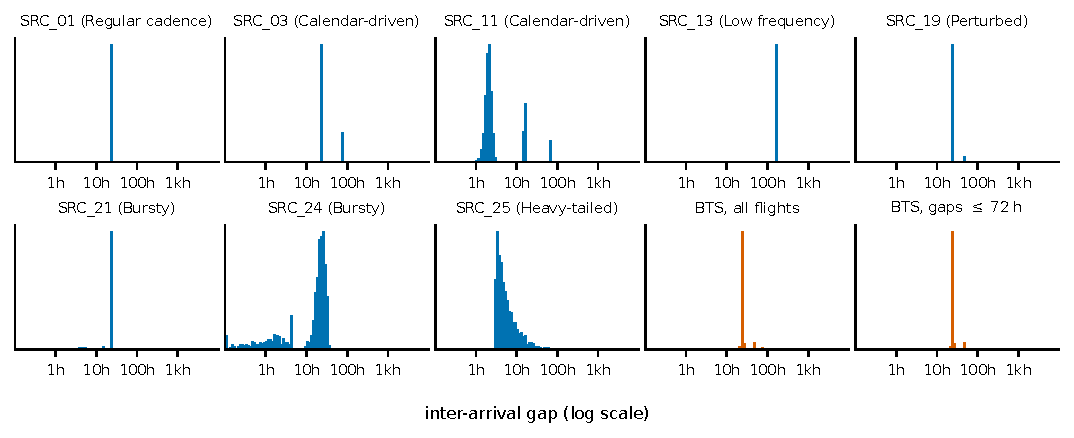
\includegraphics[width=\textwidth]{fig_data_overview.pdf}
\caption{Inter-arrival gap distributions (log scale) for eight representative synthetic sources (blue)
and for all BTS flight numbers pooled (orange; right: gaps $\le$ 72\,h). Regular sources are single
spikes; calendar-driven sources are multi-modal; bursty and heavy-tailed sources span orders of
magnitude.}
\label{fig:data}
\end{figure*}

\begin{table*}[t]
\centering\scriptsize
\caption{The 26 synthetic sources (2023--2024). Median gap in hours; $n$ = arrivals; test = completed test gaps scored. $\dagger$: fewer than 5 test events, excluded from headline statistics; SRC\_23 (annual, 2 arrivals) cannot be modelled.}
\label{tab:sources}
\begin{tabular}{llp{9.2cm}rrr}
\toprule
Source & Group & Generating pattern & $n$ & Median gap & Test \\
\midrule
SRC\_01 & Regular cadence & Daily at $\sim$09:00 UTC -- every calendar day & 731 & 24.0 & 109 \\
SRC\_02 & Calendar-driven & Daily at $\sim$09:00 UTC, $\sim$4h late on Wednesdays & 731 & 24.0 & 109 \\
SRC\_03 & Calendar-driven & Weekdays only at $\sim$14:00 UTC & 522 & 24.1 & 79 \\
SRC\_04$^\dagger$ & Low frequency & Monthly -- first business day at $\sim$06:00 UTC & 24 & 743.0 & 3 \\
SRC\_05$^\dagger$ & Low frequency & Quarterly -- first biz day of Jan/Apr/Jul/Oct at $\sim$06:00 UTC & 8 & 2184.0 & 1 \\
SRC\_06 & Calendar-driven & Tuesday, Wednesday, Thursday only at $\sim$11:00 UTC & 313 & 24.2 & 47 \\
SRC\_07 & Calendar-driven & Weekdays excluding US federal holidays at $\sim$08:00 UTC & 500 & 24.1 & 75 \\
SRC\_08 & Regular cadence & Hourly 24/7 & 17544 & 1.0 & 2631 \\
SRC\_09 & Regular cadence & Every 6 hours (00/06/12/18 UTC), every day & 2924 & 6.0 & 438 \\
SRC\_10 & Calendar-driven & Twice daily on weekdays ($\sim$08:00 and $\sim$18:00 UTC) & 1044 & 11.2 & 156 \\
SRC\_11 & Calendar-driven & Business hours every 2h on weekdays (08/10/12/14/16 UTC) & 2610 & 2.1 & 391 \\
SRC\_12 & Low frequency & Weekly -- Mondays only at $\sim$07:00 UTC & 105 & 168.0 & 15 \\
SRC\_13 & Low frequency & Weekly -- Fridays at $\sim$16:00 UTC, high jitter ($\pm$2h) & 104 & 168.1 & 15 \\
SRC\_14 & Calendar-driven & Weekdays at $\sim$09:00 UTC + reduced weekend service at $\sim$15:00 UTC & 731 & 24.0 & 109 \\
SRC\_15 & Low frequency & Bi-weekly -- alternating Mondays at $\sim$07:00 UTC & 53 & 336.0 & 8 \\
SRC\_16$^\dagger$ & Low frequency & Last business day of each month at $\sim$16:00 UTC (higher jitter) & 24 & 740.8 & 3 \\
SRC\_17 & Low frequency & 5th/15th/25th of month (or next biz day) at $\sim$09:00 UTC & 72 & 240.1 & 11 \\
SRC\_18$^\dagger$ & Low frequency & Second Tuesday of each month at $\sim$10:00 UTC & 24 & 672.3 & 3 \\
SRC\_19 & Perturbed & Daily at $\sim$10:00 UTC with 5\% random outage probability & 698 & 24.0 & 104 \\
SRC\_20 & Perturbed & Daily at $\sim$10:00 UTC -- 3x jitter in Dec and Jan & 731 & 24.0 & 109 \\
SRC\_21 & Bursty & Daily at $\sim$09:00 UTC + 3 files/day on last 3 days of quarter & 779 & 24.0 & 117 \\
SRC\_22 & Bursty & Weekdays at $\sim$09:00 UTC; 8\% chance of correction file $\sim$3h later & 570 & 24.0 & 85 \\
SRC\_23 & Low frequency & Annual -- first business day of the year at $\sim$06:00 UTC & 2 & 8735.6 & -- \\
SRC\_24 & Bursty & Self-exciting (Hawkes-like): daily background + offspring within 4h (alpha=0.4, beta=0.5/h) & 1001 & 20.5 & 150 \\
SRC\_25 & Heavy-tailed & Heavy-tail inter-arrivals: Pareto(b=1.5, scale=3h) & 2022 & 4.7 & 304 \\
SRC\_26 & Perturbed & Weekdays at $\sim$09:00 UTC; delay proportional to previous file size (LogNormal sizes, 0.5 min/MB, cap 120 min) & 522 & 24.1 & 79 \\
\bottomrule
\end{tabular}
\end{table*}


% =====================================================================
\section{Problem Formulation}\label{sec:formulation}
% =====================================================================
\subsection{Next-gap forecasting as a TPP}
For one source let $t_1<\dots<t_n$ be the arrival times observed in a window $[t_1,T]$ and
$\dt_i=t_i-t_{i-1}$ the gaps, in hours. Let $\mathcal{H}_i=\{t_1,\dots,t_i\}$ be the history. A model
defines the conditional density $p(\dt_{i+1}\mid\mathcal{H}_i)$ of the next gap, or equivalently the
intensity $\lambda^*(t)$ for $t>t_i$, with survival
$S(\tau\mid\mathcal{H}_i)=\exp\!\big(-\int_0^{\tau}\lambda^*(t_i+s)\,ds\big)$. The log-likelihood
of the window is
\begin{equation}
\label{eq:ll}
\log\mathcal{L}=\sum_{i=1}^{n-1}\log p(\dt_{i+1}\mid\mathcal{H}_i)\;+\;\log S(T-t_n\mid\mathcal{H}_n).
\end{equation}
The last term is the right-censored ``quiet tail'', which records only that no event occurred
between the last arrival and the end of observation. Setting $T=t_n$ silently drops this term and
biases every model towards gaps that are too short, so we always set $T$ to the real end of
observation.

\subsection{Splits and censoring}
Each source is split \emph{chronologically by event count} into 70\% train, 15\% validation and
15\% test; splitting by count rather than by calendar time prevents sparse sources (24 monthly
events) from ending up with an empty test set. The window of each split ends at the first event of
the next split, so that its censored tail is exactly the time until the next split's data begin, and
the test window ends at the study end (1 January 2025). Sources with fewer than five test events are
flagged \texttt{low\_n}; they are shown in figures but excluded from headline statistics, which
leaves \SynNValid{} of \SynNSources{} evaluable synthetic sources and \BtsNValid{} of \BtsNSources{}
flights.

\subsection{Covariates}
The neural models receive, for each event, nine calendar covariates computed only from the arrival
timestamp: hour of day, day of week and month, each as a sine/cosine pair, together with weekend,
business-hours and US-federal-holiday flags. The cyclical encoding places 23:00 next to 00:00, and
because nothing beyond the timestamp is used, the same features are available in real time. The
classical models, by construction, have no slot for covariates.

% =====================================================================
\section{Methods}\label{sec:methods}
% =====================================================================
\subsection{Models}
\paragraph{Poisson.} The homogeneous Poisson process has a constant intensity $\lambda$, estimated by
maximum likelihood as $\hat\lambda=n/T$, so that $\dt\sim\mathrm{Exp}(\hat\lambda)$ irrespective of
history. It serves as the reference against which all gains are measured.

\paragraph{Hawkes.} The Hawkes model has intensity $\lambda^*(t)=\mu+\alpha\sum_{t_j<t}e^{-\beta(t-t_j)}$
and branching ratio $\alpha/\beta$. Its likelihood is evaluated in $O(n)$ using the recursion
$R_i=e^{-\beta\dt_i}(1+R_{i-1})$~\citep{ozaki1979maximum} and maximised with Nelder--Mead from five
starting points, because a single start converged to a spurious $\alpha\to0$ optimum on about half of
the starting points we tried. Given the excitation state $R$ just after an event, the predictive
survival has the closed form
\begin{equation}
S(s)=\exp\!\Big(-\mu s-\tfrac{\alpha R}{\beta}\big(1-e^{-\beta s}\big)\Big).
\end{equation}

\paragraph{Neural Hawkes (\NHP).} We use a single-type continuous-time LSTM~\citep{mei2017neural} in
which, after event $i$, the cell state relaxes from $c_i$ towards a target $\bar c_i$ at learned
rates $\delta_i$:
\begin{equation}
c(t)=\bar c_i+(c_i-\bar c_i)\,e^{-\delta_i(t-t_i)},\quad h(t)=o_i\odot\tanh c(t),
\end{equation}
and $\lambda^*(t)=\mathrm{softplus}(w^\top h(t)+b)$. The input at each event is a Time2Vec embedding
(dimension 8) of the gap, scaled by the training median and concatenated with the calendar
covariates, and the cell is updated using the hidden and cell states \emph{decayed to the event
time}. The compensator within each interval is estimated by Monte Carlo with five uniform points,
whereas the predictive survival function used for evaluation is computed by trapezoidal quadrature
of $\lambda^*$ on a 300-point grid.

\paragraph{\LNM.} The intensity-free model of Shchur et al.~\citep{shchur2020intensity} uses a GRU with hidden size
$H$ that reads the standardised log-gap and the calendar covariates of each event; its state $h_i$
parameterises a $K$-component log-normal mixture
\begin{equation}
p(\dt\mid h_i)=\sum_{k=1}^{K}w_k\,\frac{1}{\dt\,\sigma_k\sqrt{2\pi}}
\exp\!\Big(-\frac{(\log\dt-\mu_k)^2}{2\sigma_k^2}\Big),
\end{equation}
with $(w,\mu,\log\sigma)$ produced by a linear head and a softmax over $w$, so that likelihood, CDF and
survival are all available in closed form; the censored tail uses the state after the last observed
gap. We cap $\sigma_k\le e$, because a looser cap ($e^5$) allowed a low-weight component to spread
mass over astronomically long gaps and made CRPS diverge, and we initialise the mixture locations at
the training mean log-gap.

\subsection{Training}\label{sec:training}
Both neural models are trained per source with Adam~\citep{kingma2015adam} (gradient-norm clip 5) and
early stopping on validation NLL (patience 20 epochs, minimum improvement $10^{-4}$), after which the
best validation weights are restored. Because sequence lengths range from tens of events to 17,544,
and a full unroll of the CT-LSTM on the hourly source took about 30\,s per gradient step, long
sequences are trained with truncated back-propagation through time (BPTT)~\citep{williams1990efficient}.
Each window holds about 128 events and is preceded by 32 burn-in events that warm up the recurrent
state without contributing to the loss, and windows are shuffled and batched 16 at a time. Sequences
shorter than 256 events form a single window and use the exact objective of Eq.~\eqref{eq:ll},
including the censored tail. Two initialisations stabilise training: \NHP{} starts with its intensity
bias at the training rate ($\mathrm{softplus}(b)=1/\overline{\dt}$), and \LNM{} standardises its
log-gap input with training statistics. All runs use a single CPU thread and fixed seeds, with \LNM{}
trained over \SynLogNormMixSeeds{} seeds and \NHP{} over \SynNHPSeeds{}.

\subsection{Hyper-parameter selection}
Configurations are compared on \emph{validation} NLL only, using the synthetic sources with at least
ten validation events. For each source we average the best validation loss over seeds and take its
difference from a reference configuration; a candidate replaces the reference only if the mean
difference is more than two standard errors below zero, and otherwise it is treated as a tie and the
cheaper setting is kept. Table~\ref{tab:tuning} lists the candidates. Because validation losses are
comparable only between runs with the same windowing, window length and burn-in were held fixed.

\subsection{Evaluation}
Each test event is scored with the model state replayed through \emph{all} preceding events, namely
the Hawkes excitation $R$ and the GRU or CT-LSTM state carried through the full train+validation
history; resetting the state at the test boundary would discard exactly the information the models
are meant to exploit. Every model exposes only \texttt{cdf()} and \texttt{log\_prob()}, and all
metrics are computed from these two functions:
\begin{itemize}
\item \textbf{NLL}: mean $-\log p(\dt)$ over completed test gaps (nats, time in hours).
\item \textbf{CRPS}: $\int_0^\infty(F(t)-\mathbb{1}[t\ge y])^2dt$~\citep{matheson1976scoring}, by
  adaptive log-spaced quadrature with controlled tail error. The same estimator is applied to every
  model, so that none benefits from a closed-form shortcut, and it agrees with the closed form for
  exponential distributions to within 0.2\%.
\item \textbf{PICP}: observed coverage of the central 50/80/90\% predictive intervals, together with
  PIT histograms~\citep{dawid1984present}.
\item \textbf{MAE / lag-1}: MAE of the predictive median divided by the MAE of the naive ``same gap
  as last time'' forecast.
\end{itemize}
Because raw NLL and CRPS scale with a source's cadence, cross-source summaries use the \emph{NLL
gain} over Poisson, $\nll_{\text{Poisson}}-\nll_{\text{model}}$ (nats/event, invariant to the time
unit), and the \emph{CRPS skill} $1-\crps/\crps_{\text{Poisson}}$. Models are compared with paired
Wilcoxon signed-rank tests across sources~\citep{wilcoxon1945individual}; since the sources were
designed rather than sampled, the resulting $p$-values should be read as descriptive.

\subsection{System design}
The study is implemented as an installable Python package (PyTorch~\citep{paszke2019pytorch}) with a
single command-line entry point. It comprises a data pipeline (synthetic generator and BTS
extractor), a resumable experiment runner that caches each (source, model, seed) unit, and
an inference module.

% =====================================================================
\section{Results}\label{sec:results}
% =====================================================================
\subsection{Hyper-parameter selection}
Table~\ref{tab:tuning} summarises the search. For \LNM{}, lowering the learning rate to
$3\cdot10^{-3}$ improved validation NLL on 17 of 20 sources ($\Delta=-0.255\pm0.050$), whereas a
larger hidden state or eight mixture components were slightly worse. For \NHP{} the lower learning
rate was worse on 18 of 20 sources and hit the epoch cap more often, so the reference rate
$10^{-2}$ was kept together with a larger epoch budget (600). The final configuration, $H=32$, $K=4$
and $\eta_{\text{LNM}}=3\cdot10^{-3}$, was frozen before any BTS result was computed.

\begin{table}[t]
\centering\small
\caption{Hyper-parameter selection on the \emph{validation} split only (synthetic sources with $\geq$10 validation events). $\Delta$ is the mean change in validation NLL per event relative to the reference ($<0$ is better), with its standard error over sources.}
\label{tab:tuning}
\resizebox{\columnwidth}{!}{%
\begin{tabular}{llccccc}
\toprule
Model & Configuration & $\Delta$ val.\ NLL & SE & Better on & At cap & Seeds \\
\midrule
LogNormMix & reference ($\eta=10^{-2}$, $H=32$, $K=4$) & 0 & -- & -- & 0.01 & 10 \\
LogNormMix & $\eta=3\cdot10^{-3}$ & -0.255 & 0.050 & 17/20 & 0.12 & 10 \\
LogNormMix & hidden size $H=64$ & +0.089 & 0.047 & 7/20 & 0.01 & 10 \\
LogNormMix & $K=8$ mixture components & +0.086 & 0.035 & 6/20 & 0.01 & 10 \\
\midrule
NHP & reference ($\eta=10^{-2}$, $H=32$) & 0 & -- & -- & 0.08 & 3 \\
NHP & $\eta=3\cdot10^{-3}$ & +0.183 & 0.038 & 2/20 & 0.22 & 3 \\
\bottomrule
\end{tabular}}
\end{table}


\subsection{Synthetic sources}\label{sec:syn-results}
\begin{table*}[t]
\centering\small
\caption{Synthetic sources: test-set results over 21 sources (medians over sources; neural models averaged over seeds first). NLL gain = $\mathrm{NLL}_{\text{Poisson}} - \mathrm{NLL}_{\text{model}}$ in nats/event; CRPS skill = $1-\mathrm{CRPS}/\mathrm{CRPS}_{\text{Poisson}}$; mean rank by NLL (1 = best); MAE / lag-1 is the ratio of the median-forecast MAE to the naive last-gap forecast ($<1$ is better). Best value per column in bold.}
\label{tab:scoreboard-syn}
\begin{tabular}{lcccccccc}
\toprule
 & \multicolumn{2}{c}{Probabilistic skill} & & \multicolumn{2}{c}{Sources won} & \multicolumn{2}{c}{Interval coverage} & Point \\
\cmidrule(lr){2-3}\cmidrule(lr){5-6}\cmidrule(lr){7-8}\cmidrule(lr){9-9}
Model & NLL gain & CRPS skill & Mean rank & NLL & CRPS & 50\% & 80\% & MAE / lag-1 \\
\midrule
Poisson & +0.00 & 0.00 & 3.57 & 0/21 & 0/21 & 0.94 & 1.00 & 2.15 \\
Hawkes & +0.00 & 0.00 & 3.43 & 0/21 & 0/21 & 0.94 & 1.00 & 2.15 \\
NHP & +1.76 & \textbf{0.80} & 1.95 & 1/21 & 10/21 & 0.91 & 1.00 & 0.59 \\
LogNormMix & \textbf{+3.31} & 0.76 & \textbf{1.05} & 20/21 & 11/21 & 0.49 & 0.81 & \textbf{0.50} \\
\bottomrule
\end{tabular}
\end{table*}


Table~\ref{tab:scoreboard-syn} gives the test-set scoreboard over the \SynNValid{} evaluable
synthetic sources (\SynNTestEvents{} test gaps). Both neural models beat Poisson in NLL on every
source, and \LNM{} is the clear NLL winner, with the lowest NLL on \SynLogNormMixBestNLL{} of
\SynNValid{} sources, a median gain of \SynLogNormMixGain{} nats/event over Poisson and a mean rank of
\SynLogNormMixRank. Against \NHP{} it is better on \SynNllLogNormMixVsNHPWins{} sources, by a median
of \SynNllLogNormMixVsNHPEffect{} nats/event (Table~\ref{tab:paired}).

CRPS ranks the two neural models differently: \NHP{} wins \SynNHPBestCRPS{} sources and \LNM{}
\SynLogNormMixBestCRPS{}, their median skills are \SynNHPSkill{} and \SynLogNormMixSkill{}, and the
paired test cannot separate them ($p=\SynCrpsLogNormMixVsNHPP$). Figure~\ref{fig:heatmap} shows where
the disagreement arises. On most calendar-driven sources (SRC\_02--SRC\_11) and on SRC\_21, 22 and
26, \NHP{} has the better CRPS but the worse NLL, because its predictive distributions are wide but
well centred, which CRPS rewards. \LNM{} instead concentrates its mass sharply on the dominant mode,
which NLL rewards but which costs CRPS whenever an occasional gap falls in a minor mode.

The Hawkes process adds nothing. Its NLL gain over Poisson rounds to zero on every source except
SRC\_11 (business-hours bursts, +0.1), and its CRPS departs from Poisson's only on SRC\_24 (the
Hawkes-generated source) and SRC\_25 (Pareto gaps), where it is slightly worse
(Figure~\ref{fig:heatmap}). Even on SRC\_24, which was generated by a self-exciting mechanism, it
gains nothing in NLL; Section~\ref{sec:hawkes} shows that this reflects a model mismatch rather than
a fitting error.

\begin{figure*}[t]
\centering
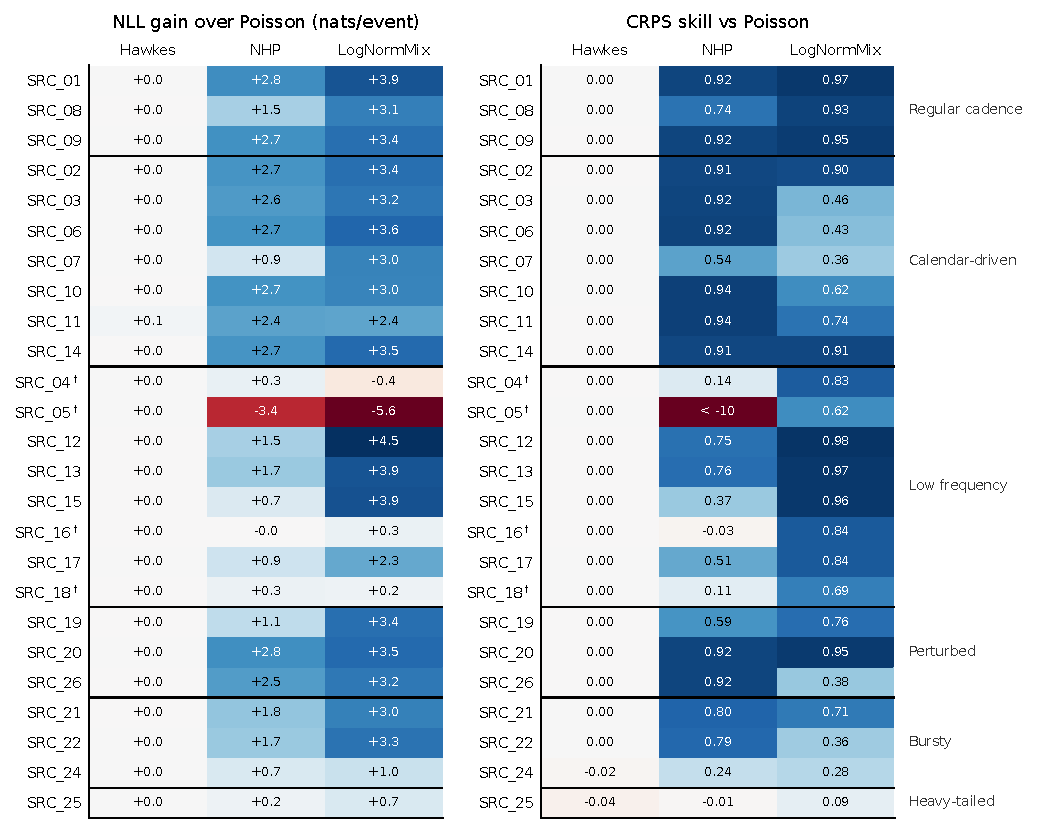
\includegraphics[width=0.78\textwidth]{fig_gain_heatmap.pdf}
\caption{Per-source NLL gain (left) and CRPS skill (right) over Poisson on synthetic data, grouped by
schedule type. Blue is better than Poisson. $\dagger$: \texttt{low\_n} sources (excluded from headline
statistics). On quarterly SRC\_05 (8 events, 1 test event) both neural models overfit.}
\label{fig:heatmap}
\end{figure*}

\begin{table}[t]
\centering\small
\caption{Median NLL gain over Poisson (nats/event) by schedule type, synthetic data.}
\label{tab:groups}
\begin{tabular}{lccc}
\toprule
Schedule type & Sources & NHP & LogNormMix \\
\midrule
Regular cadence & 3 & +2.74 & +3.40 \\
Calendar-driven & 7 & +2.67 & +3.24 \\
Low frequency & 4 & +1.23 & +3.90 \\
Perturbed & 3 & +2.51 & +3.38 \\
Bursty & 3 & +1.66 & +3.03 \\
Heavy-tailed & 1 & +0.22 & +0.69 \\
\bottomrule
\end{tabular}
\end{table}


\paragraph{By schedule type.} Table~\ref{tab:groups} breaks the NLL gain down by group. \LNM{} gains
about 3--4 nats/event on every structured group and is strongest on low-frequency sources, which is
precisely where \NHP{} is weakest (+1.23): on the monthly SRC\_04 and SRC\_16 and the bi-weekly
SRC\_15, \NHP's validation loss never improved after the first epoch for several seeds, so the model
remained close to its Poisson-like initialisation. \LNM{}, for its part, overfit SRC\_05
(Figure~\ref{fig:heatmap}). The only source on which neither model gains much is
the heavy-tailed SRC\_25 (+0.22 and +0.69): with i.i.d.\ Pareto gaps there is no history to exploit,
and \LNM{} gains only by fitting the marginal shape better than an exponential.

\begin{table*}[t]
\centering\small
\caption{Paired comparisons across sources (Wilcoxon signed-rank). ``Effect'' is the median NLL advantage of A in nats/event for NLL and the median CRPS ratio A/B for CRPS ($<1$ favours A). $p$-values are descriptive: the synthetic sources are designed scenarios, not a random sample.}
\label{tab:paired}
\begin{tabular}{llcccccc}
\toprule
Metric & Comparison (A vs B) & \multicolumn{3}{c}{Synthetic} & \multicolumn{3}{c}{BTS flights} \\
\cmidrule(lr){3-5}\cmidrule(lr){6-8}
 & & A wins & Effect & $p$ & A wins & Effect & $p$ \\
\midrule
NLL & LogNormMix vs NHP & 20/21 & +0.89 & $<$0.001 & 31/34 & +1.79 & $<$0.001 \\
NLL & LogNormMix vs Poisson & 21/21 & +3.31 & $<$0.001 & 32/34 & +2.35 & $<$0.001 \\
NLL & NHP vs Poisson & 21/21 & +1.76 & $<$0.001 & 22/34 & +0.55 & 0.566 \\
NLL & Hawkes vs Poisson & 12/21 & +0.00 & 0.539 & 23/34 & +0.00 & 0.091 \\
\midrule
CRPS & LogNormMix vs NHP & 11/21 & 0.943 & 0.946 & 31/34 & 0.695 & $<$0.001 \\
CRPS & LogNormMix vs Poisson & 21/21 & 0.239 & $<$0.001 & 34/34 & 0.315 & $<$0.001 \\
CRPS & NHP vs Poisson & 20/21 & 0.203 & $<$0.001 & 28/34 & 0.540 & $<$0.001 \\
CRPS & Hawkes vs Poisson & 9/21 & 1.000 & 0.089 & 20/34 & 1.000 & 0.309 \\
\bottomrule
\end{tabular}
\end{table*}


\subsection{Calibration}
Figure~\ref{fig:calibration} and the PIT histograms in Figure~\ref{fig:pit} reveal the starkest
difference between the models. \LNM{} is close to calibrated, with median observed coverage of
\SynLogNormMixCovFifty{}, \SynLogNormMixCovEighty{} and \SynLogNormMixCovNinety{} at the 50, 80 and
90\% levels and a nearly flat PIT histogram. The three intensity-based models, by contrast, are
severely under-confident: their 50\% intervals cover \SynNHPCovFifty--\SynPoissonCovFifty{} of
outcomes, their 80\% intervals essentially all of them, and their humped PIT histograms show that the
true gaps sit in the middle of distributions that are far too wide. For Poisson and Hawkes this is
structural, since an exponential distribution with the correct mean is far wider than a
near-deterministic daily schedule. For \NHP{} it reflects the difficulty of forming a sharp, unimodal density from an
intensity that must first rise from near zero and then fall, within a softplus-of-linear head.

\begin{figure*}[t]
\centering
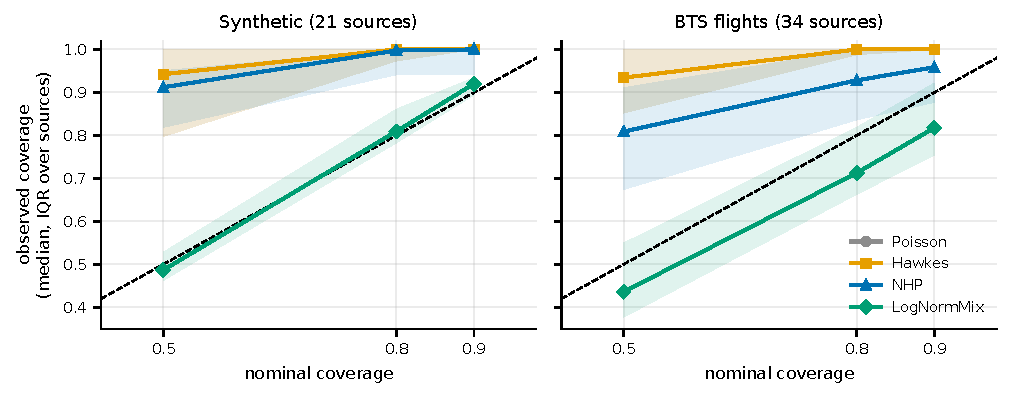
\includegraphics[width=0.85\textwidth]{fig_calibration.pdf}
\caption{Reliability of the central predictive intervals (median and inter-quartile range over sources).
Points on the diagonal are calibrated; points above it are too wide (under-confident). Only \LNM{} is
close to calibrated; on BTS it becomes moderately over-confident.}
\label{fig:calibration}
\end{figure*}

\begin{figure}[t]
\centering
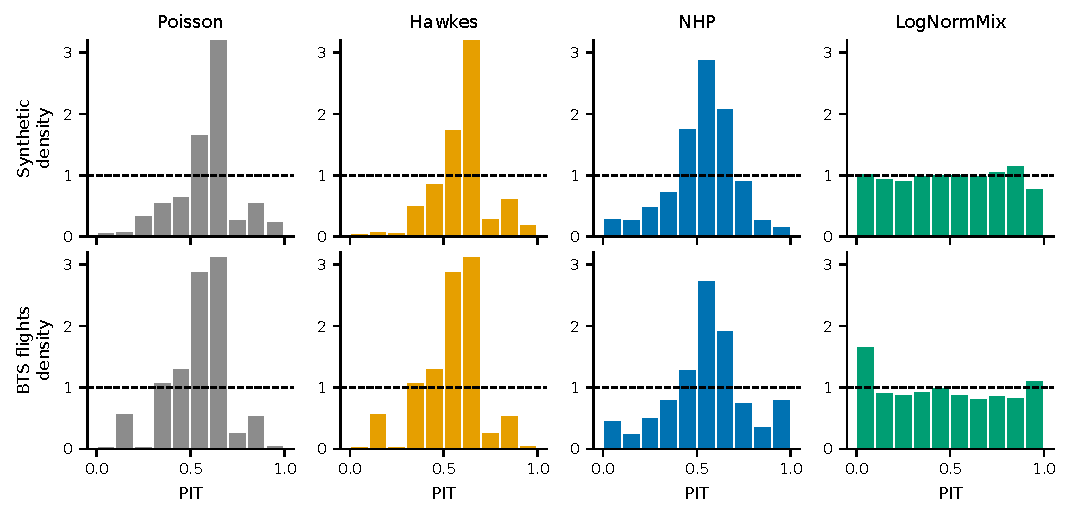
\includegraphics[width=\columnwidth]{fig_pit.pdf}
\caption{PIT histograms (equal weight per source). Flat = calibrated; a central hump = intervals too
wide; mass at the edges = too narrow.}
\label{fig:pit}
\end{figure}

\subsection{Point forecasts}
Operational users often want a single predicted time rather than a distribution. Taking the predictive median as the
point forecast and comparing its MAE with that of the naive ``same gap as last time'' (lag-1) rule,
the median ratio is \SynLogNormMixMaeRatio{} for \LNM{}, 0.59 for \NHP{} and 2.15 for Poisson and
Hawkes (Table~\ref{tab:scoreboard-syn}). \LNM{} beats the lag-1 rule on \SynLogNormMixBeatsLag{} of
\SynNValid{} sources and \NHP{} on \SynNHPBeatsLag{},
whereas Poisson and Hawkes beat it on only \SynPoissonBeatsLag{} (Figure~\ref{fig:mae}). The
classical models lose mainly on near-regular feeds: for a daily file the exponential median is
$24\ln 2\approx16.6$\,h, about 7.4\,h off every time, whereas repeating the last gap is nearly exact.
On point accuracy the two neural models are close.

Table~\ref{tab:group-mae} explains why the overall medians are so close. \NHP{} makes the sharper
single guess on calendar-driven (0.50 vs.\ 4.22\,h), bursty and perturbed feeds, the schedules whose
next gap is set by the calendar, whereas \LNM{} is far more accurate on low-frequency feeds (2.81
vs.\ 19.03\,h) and on the heavy-tailed feed. On low-frequency feeds, simply repeating the last gap
(2.07\,h) beats both neural models, which makes it a useful default for sources with little history.
Because each group holds only one to seven sources, these differences should be read as patterns
rather than firm conclusions.

\begin{table}[t]
\centering\small
\caption{Median MAE (hours) of the median forecast by schedule type, synthetic data. ``Lag-1'' repeats the previous gap. Hawkes is omitted (within 0.3\,h of Poisson in every group). Lowest value per row in bold.}
\label{tab:group-mae}
\resizebox{\columnwidth}{!}{%
\begin{tabular}{lccccc}
\toprule
Schedule type & $n$ & Poisson & NHP & LogNormMix & Lag-1 \\
\midrule
Regular cadence & 3 & 1.84 & 0.11 & \textbf{0.10} & 0.21 \\
Calendar-driven & 7 & 7.37 & \textbf{0.50} & 4.22 & 13.91 \\
Low frequency & 4 & 63.41 & 19.03 & 2.81 & \textbf{2.07} \\
Perturbed & 3 & 7.94 & \textbf{1.04} & 1.64 & 3.12 \\
Bursty & 3 & 11.23 & \textbf{2.56} & 7.16 & 13.70 \\
Heavy-tailed & 1 & 4.59 & 4.97 & \textbf{4.26} & 7.38 \\
\bottomrule
\end{tabular}}
\end{table}


Figure~\ref{fig:example} illustrates the practical difference on the outage-prone SRC\_19: Poisson's
50\% interval spans roughly 7--35\,h for a file that arrives about every 24\,h, whereas \LNM's is
well under an hour wide. Neither model anticipates the random outages (the two 48\,h gaps), which are
unpredictable by construction.

\begin{figure*}[t]
\centering
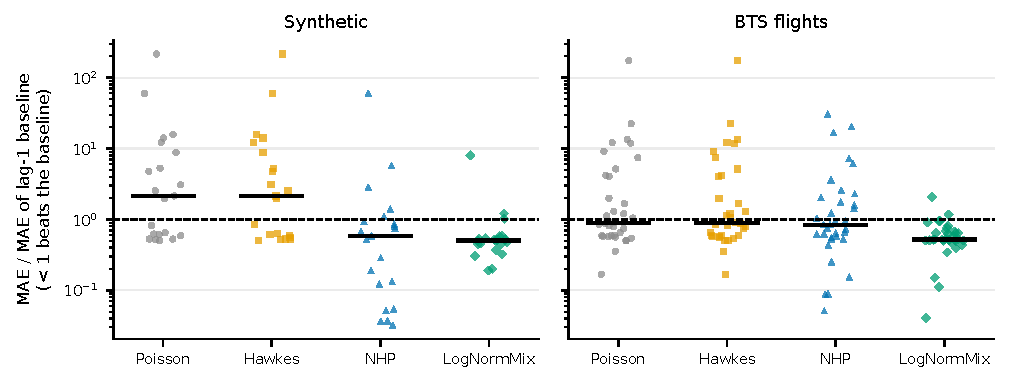
\includegraphics[width=0.85\textwidth]{fig_mae_ratio.pdf}
\caption{MAE of the median forecast relative to the lag-1 baseline, one point per source (log scale;
bar = median). Below 1 beats ``same gap as last time''.}
\label{fig:mae}
\end{figure*}

\begin{figure*}[t]
\centering
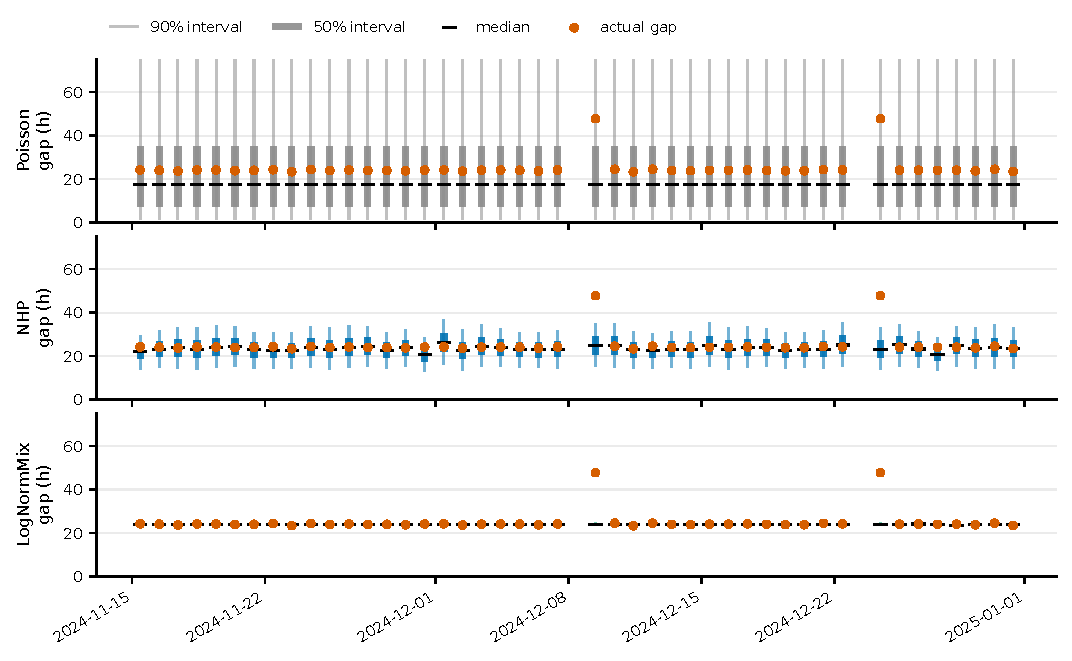
\includegraphics[width=0.85\textwidth]{fig_example_forecast.pdf}
\caption{Last 45 test forecasts for SRC\_19 (daily at 10:00 with 5\% random outages; seed 0). Bars:
50\% (thick) and 90\% (thin) predictive intervals; dash: median; dots: actual gap.}
\label{fig:example}
\end{figure*}

\subsection{Held-out check on real flight arrivals}
\begin{table*}[t]
\centering\small
\caption{BTS flight arrivals (held-out check, settings frozen from the synthetic study): test-set results over 34 flight numbers. Columns as in Table~\ref{tab:scoreboard-syn}.}
\label{tab:scoreboard-bts}
\begin{tabular}{lcccccccc}
\toprule
 & \multicolumn{2}{c}{Probabilistic skill} & & \multicolumn{2}{c}{Sources won} & \multicolumn{2}{c}{Interval coverage} & Point \\
\cmidrule(lr){2-3}\cmidrule(lr){5-6}\cmidrule(lr){7-8}\cmidrule(lr){9-9}
Model & NLL gain & CRPS skill & Mean rank & NLL & CRPS & 50\% & 80\% & MAE / lag-1 \\
\midrule
Poisson & +0.00 & 0.00 & 3.26 & 0/34 & 0/34 & 0.93 & 1.00 & 0.89 \\
Hawkes & +0.00 & 0.00 & 2.91 & 2/34 & 0/34 & 0.93 & 1.00 & 0.89 \\
NHP & +0.55 & 0.46 & 2.62 & 3/34 & 3/34 & 0.81 & 0.93 & 0.84 \\
LogNormMix & \textbf{+2.35} & \textbf{0.69} & \textbf{1.21} & 29/34 & 31/34 & 0.44 & 0.71 & \textbf{0.52} \\
\bottomrule
\end{tabular}
\end{table*}


Table~\ref{tab:scoreboard-bts} applies the frozen configuration to the \BtsNValid{} evaluable
flight numbers, and \LNM's advantage not only carries over but widens.
It has the lowest NLL on \BtsLogNormMixBestNLL{} of \BtsNValid{} flights and the lowest CRPS on
\BtsLogNormMixBestCRPS{}, with a median NLL gain of \BtsLogNormMixGain{} nats/event and a CRPS skill
of \BtsLogNormMixSkill{}; it beats \NHP{} on \BtsNllLogNormMixVsNHPWins{} flights in NLL and
\BtsCrpsLogNormMixVsNHPWins{} in CRPS ($p<0.001$ for both), and it beats the lag-1 forecast on
\BtsLogNormMixBeatsLag{} of \BtsNValid{} flights (Figure~\ref{fig:mae}). \NHP{} degrades much more: its median gain over
Poisson falls to \BtsNHPGain{} nats/event, and it is better than Poisson on only
\BtsNllNHPVsPoissonWins{} flights, a difference that is not significant ($p=\BtsNllNHPVsPoissonP$;
Figure~\ref{fig:bts}). Hawkes again collapses to Poisson.

In point accuracy, \LNM's median MAE ratio to the lag-1 rule is 0.52 on flights against 0.84 for
\NHP{} (Table~\ref{tab:scoreboard-bts}); on real data, therefore, the near-tie seen on synthetic
sources is broken in \LNM's favour. \NHP's failures are concentrated on a few flights, on several of
which it is more than one nat worse than Poisson (Figure~\ref{fig:bts}). Flight numbers have short
histories, and one plausible explanation, which we have not tested directly, is that the larger
CT-LSTM has too little data to learn a robust intensity.

\LNM's calibration also shifts on flights, where its intervals become moderately
\emph{over}-confident (80\% coverage \BtsLogNormMixCovEighty{}) and its PIT histogram has excess mass
at the left edge, indicating that some gaps are shorter than predicted (Figure~\ref{fig:pit}). The
likely cause is schedule changes within the test period, such as departure-time shifts, which a
model trained on the first 70\% of a flight's history has not seen; a recalibration step on recent
data would address this (Section~\ref{sec:discussion}).

\begin{figure*}[t]
\centering
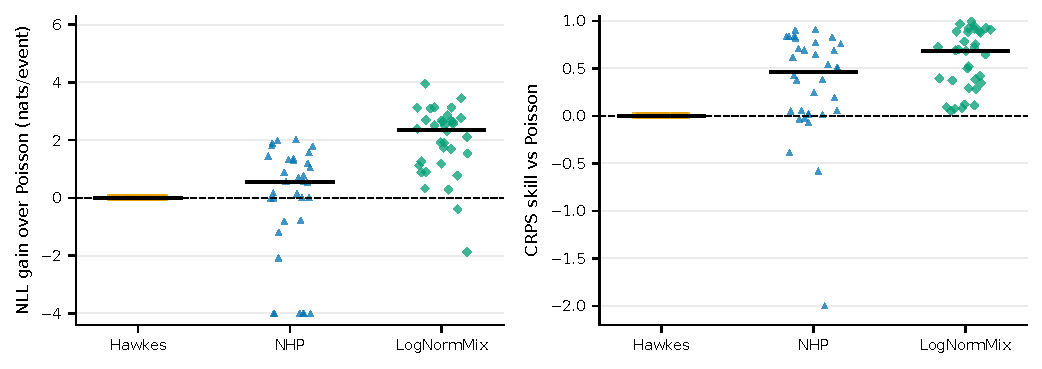
\includegraphics[width=0.85\textwidth]{fig_bts_gain.pdf}
\caption{BTS flights: per-flight NLL gain and CRPS skill over Poisson (points clipped to the axis
range; bar = median). \NHP{} is better than Poisson on most flights but loses heavily on a few.}
\label{fig:bts}
\end{figure*}

\subsection{Where models fail: unusually long gaps}\label{sec:long-gaps}
Average scores can hide failures on rare events, and for monitoring it is precisely the rare long
gaps that matter. Figure~\ref{fig:gaps} therefore splits test gaps by their length relative to the
source's median gap. On synthetic data both neural models retain a large gain on long gaps
($>2\times$ the median: \SynGapBinLogNormMixVeryLong{} for \LNM, \SynGapBinNHPVeryLong{} for \NHP),
but on flights, where long gaps arise from cancellations and suspended services, \NHP{} collapses
(\BtsGapBinNHPVeryLong{} nats/event). Its learned intensity decays almost to zero after the usual
24\,h, so a multi-day gap receives a vanishing survival probability. \LNM{} also loses to Poisson on
these gaps (\BtsGapBinLogNormMixVeryLong{}), but by an order of magnitude less, because its mixture
retains a wide component. This failure mode accounts for \NHP's weak aggregate result on BTS and, for
production use, argues for an explicit ``outage'' component or robust mixing with a heavy-tailed
fallback.

\begin{figure*}[t]
\centering
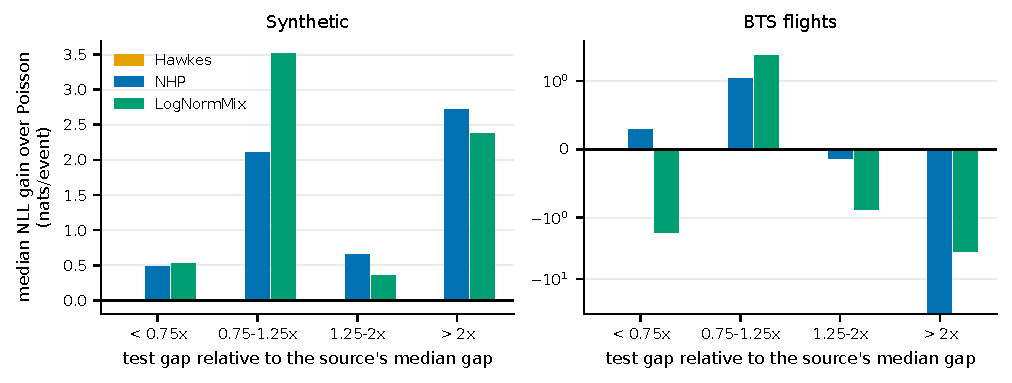
\includegraphics[width=0.85\textwidth]{fig_gap_bins.pdf}
\caption{Median NLL gain over Poisson by test-gap length relative to the source's median gap (BTS panel
on a symlog scale). On flights, \NHP{} fails catastrophically on gaps longer than twice the usual gap.}
\label{fig:gaps}
\end{figure*}

\subsection{Why the Hawkes process finds no self-excitation}\label{sec:hawkes}
SRC\_24 was generated to be self-exciting: it has one main file per day at a random time, each main
file triggers a single follow-up within four hours with probability 0.4, and follow-ups trigger no
further files. Counted over the realised data, the true number of follow-ups per file, which is the
quantity comparable to the branching ratio $\alpha/\beta$, is \HkTrueRatio. The fitted Hawkes
process nevertheless estimates only \HkFitRatio, and we ran two checks to rule out an
implementation error (Figure~\ref{fig:hawkes}).

In a recovery experiment, we simulated \HkSimN{} feeds of the same size as SRC\_24 from an exponential-kernel Hawkes process with a \emph{constant} background and a true
branching ratio of \HkSimTrue; the same fitting code recovers this value, with a mean estimate of
\HkSimMean{} and a range of \HkSimMin--\HkSimMax. A profile likelihood, obtained by fixing the
branching ratio on a grid and maximising over $(\mu,\beta)$, shows that SRC\_24's training likelihood
peaks at about \HkProfileBest{} and is \HkProfileDeltaTrue{} log-likelihood units lower at the design
value of \HkTrueRatio. The low estimate is therefore what the data support \emph{under this model},
not a local optimum.

The cause lies in the background. The Hawkes model assumes that main files arrive at random, whereas
SRC\_24's main files arrive like clockwork, once a day. A memoryless background at the fitted rate
would by chance already produce many gaps shorter than four hours, so the model attributes most short
gaps to chance and has little left to explain through excitation. The same mismatch plausibly explains the
collapse on flights, which also follow a daily schedule; a Hawkes process with a calendar-dependent
background $\mu(t)$ would be the natural remedy, and we leave it to future work.

\begin{figure*}[t]
\centering
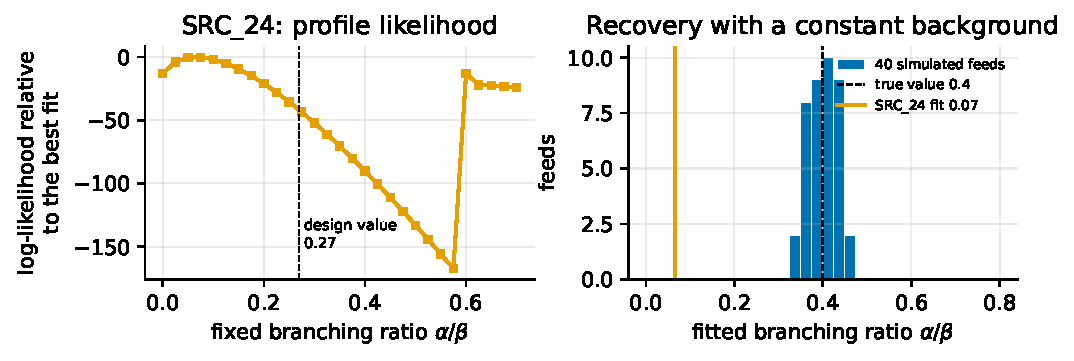
\includegraphics[width=0.85\textwidth]{fig_hawkes_check.pdf}
\caption{Diagnosing the Hawkes fit on SRC\_24. Left: profile log-likelihood of the training split
as a function of a fixed branching ratio (relative to the best fit); the dashed line is the design
value. Right: branching ratios fitted to \HkSimN{} simulated feeds with a constant background and
true ratio \HkSimTrue{}, against the SRC\_24 fit. The code recovers self-excitation when the
background is random, but not when it is periodic.}
\label{fig:hawkes}
\end{figure*}

\subsection{Cost and stability}
\begin{table}[t]
\centering\small
\caption{Training cost and convergence of the neural models (CPU, one thread). ``At cap'' counts runs that were still improving when the epoch budget ran out.}
\label{tab:training}
\resizebox{\columnwidth}{!}{%
\begin{tabular}{llcccc}
\toprule
Data & Model & Runs & At cap & Best epoch & Sec./run \\
\midrule
Synthetic & NHP & 125 & 8 & 156 & 37.2 \\
Synthetic & LogNormMix & 250 & 28 & 74 & 4.3 \\
BTS & NHP & 235 & 0 & 69 & 4.1 \\
BTS & LogNormMix & 440 & 16 & 50 & 1.5 \\
\bottomrule
\end{tabular}}
\end{table}

Table~\ref{tab:training} reports training cost. A synthetic \NHP{} run takes a median of
\SynNHPSecPerRun\,s against \SynLogNormMixSecPerRun\,s for \LNM{}. The difference stems from the sequential CT-LSTM loop and the Monte
Carlo compensator, both of which \LNM{} avoids. Because \SynNHPHitCap{} \NHP{} and
\SynLogNormMixHitCap{} \LNM{} runs ended at the epoch cap, a few models may be slightly
under-trained.

% =====================================================================
\section{Discussion and Limitations}\label{sec:discussion}
% =====================================================================
\paragraph{Main findings.} Five findings emerge from the study. First, regular schedules are not
memoryless: both neural models improve on Poisson by 2--4 nats/event, which corresponds to
predictive densities that are on average (geometric mean) $e^{2}$--$e^{4}$ times higher at the
observed gap. Second, on this kind of data an intensity-free density model is the better inductive
bias. \LNM{} wins on likelihood, calibration and cost, ties \NHP{} on point accuracy on synthetic
data while beating it on flights, and transfers to real data without re-tuning, although it becomes
somewhat over-confident there. Third, proper scores can disagree. CRPS rated \NHP{} as good as \LNM{}
on synthetic data, while NLL and PIT revealed that \NHP's distributions are much too wide, so
reporting both scores alongside calibration was necessary to reach the right conclusion. Fourth,
classical self-excitation is the wrong mechanism for calendar-driven feeds: the Hawkes process
reduces to Poisson because its constant background absorbs the short gaps that a periodic schedule
produces, even when genuine follow-up files exist (Section~\ref{sec:hawkes}). Fifth, the two neural
models have complementary strengths, with \NHP{} giving sharper point forecasts on calendar-driven and
bursty feeds and \LNM{} proving more reliable on sparse and real-world sources.

\paragraph{Implications for data-ingestion teams.}
\begin{itemize}
\item \emph{Use \LNM{} as the default forecaster.} It was the best or tied-best model on both data
  sets and trains about nine times faster than \NHP{}, which matters when models are refitted as
  sources are added or change.
\item \emph{Do not alert from constant-rate or simple self-exciting models on scheduled feeds.} Their
  typical errors are about four times (synthetic) and three times (flights) those of \LNM{}, and
  because their 80\% intervals contain essentially every arrival, an interval-based alert would
  almost never fire and late files would be noticed late.
\item \emph{Check each source's intervals before alerting on them.} On flights, \LNM's 90\% interval
  held a median of \BtsLogNormMixCovNinety{} of arrivals, which implies roughly 1.8 times the intended
  volume of out-of-range flags, some of them for \emph{early} arrivals. Observed coverage on a recent
  window should therefore be compared with the target, and the intervals recalibrated, before they
  drive alerts.
\item \emph{Use a simple rule for new or low-volume sources.} \SynNLowN{} of 25 synthetic sources and
  \BtsNLowN{} of 48 flights could not even be scored, and on low-frequency feeds repeating the last
  gap beat both neural models (Table~\ref{tab:group-mae}). Such a rule, or the conditional SLA
  probability from a model refitted as history accumulates, is the safer starting point.
\item \emph{Keep \NHP{} as a specialist} for a few high-value calendar-driven feeds, where its sharper
  point forecasts matter and its training cost is affordable.
\end{itemize}

\paragraph{Limitations.} The study has several limitations. Hyper-parameters and design choices were
made on designed synthetic scenarios, and although the BTS check guards against over-fitting to
them, the flights represent a single domain, carrier and route. Each source is also modelled
independently, so sources with only a few dozen events, such as monthly reports, are where every
model struggles and where pooling across sources would most likely help; \SynNLowN{} synthetic
sources and \BtsNLowN{} flights have fewer than five test events and are excluded from headline
statistics altogether. The chronological split realistically exposes models to schedule changes they
have not seen, which shows up as over-confidence on BTS, and we neither retrain nor recalibrate
online. Classical models without covariates are the natural reference for TPPs, but a calendar-aware
classical baseline, such as a piecewise-constant Poisson process or a seasonal empirical quantile,
would be a stronger non-neural competitor. Finally, although the runner supports removing the
calendar features and Time2Vec, the ablation runs were not completed within the project's compute
budget, so the contribution of each input has not been isolated.

% =====================================================================
\section{Conclusion}\label{sec:conclusion}
% =====================================================================
We framed ``when will the next file arrive?'' as probabilistic forecasting with temporal point
processes and compared Poisson, Hawkes, Neural Hawkes and log-normal-mixture models under a
leakage-safe, censoring-aware protocol. An intensity-free GRU with a log-normal-mixture decoder was
the most accurate model in likelihood and the only well-calibrated one. Its median gain over Poisson
was \SynLogNormMixGain{} nats/event on 21 synthetic schedules and \BtsLogNormMixGain{} on 34 real
flights, and it beat the naive lag-1 forecast on most sources while costing about nine times less
per training run than the Neural Hawkes process on the synthetic data. The Neural Hawkes process was
competitive in CRPS and gave the sharpest point forecasts on calendar-driven synthetic feeds, but it
was under-confident and fragile on unusually long gaps and on short real histories. The classical
Hawkes process offered no improvement over Poisson, and a recovery experiment together with a
profile likelihood shows that this is because a constant background cannot represent a periodic
schedule, not because the fit is wrong. For production data-pipeline monitoring we recommend the log-normal-mixture model with calendar covariates, wrapped with conditional
``still-arrives-before-deadline'' probabilities and rolling calibration checks.

\paragraph{Future work.} Natural next steps are: (i) global models trained across sources with
source embeddings; (ii) online recalibration, for example conformal or isotonic recalibration on a
recent window, to handle schedule drift; (iii) an explicit outage or mixture-with-uniform component
for robustness to rare long gaps; (iv) a Hawkes process with a calendar-dependent background, which
should recover the follow-up structure that the constant-background model misses; (v) the
calendar-feature and Time2Vec ablations and a calendar-aware classical baseline; (vi) repeating the
flight analysis on other routes and carriers to see whether \LNM's over-confidence on flights
generalises; and (vii) a cost-based alerting rule evaluated on real
incident logs.

\small
\bibliographystyle{unsrtnat}
\bibliography{refs}

\end{document}
